%%%%%%%%%%%%%%%%%%%%%%%%%%%%%%%%%%%%%%%%%
% Beamer Presentation
% LaTeX Template
% Version 1.0 (10/11/12)
%
% This template has been downloaded from:
% http://www.LaTeXTemplates.com
%
% License:
% CC BY-NC-SA 3.0 (http://creativecommons.org/licenses/by-nc-sa/3.0/)
%
%%%%%%%%%%%%%%%%%%%%%%%%%%%%%%%%%%%%%%%%%

\documentclass{beamer}
\usepackage{lmodern,textpos,hyperref,graphicx,booktabs}
\usepackage[ddmmyyyy]{datetime}

\mode<presentation> {
\usetheme{Dresden}
\usecolortheme{beaver}

\definecolor{stanfordBeige5}{RGB}{251,249,249}
\definecolor{stanfordRed}{RGB}{140,21,21}
\definecolor{stanfordBlack}{RGB}{46,45,41}
\definecolor{stanfordRedText}{RGB}{132, 0, 0}
\setbeamercolor{institute in head/foot}{fg=stanfordRedText}
\setbeamercolor*{palette tertiary}{use=structure,fg=white,bg=stanfordRed}
}

\title[Worker--Centric Markets]{Designing Worker--Centric Labor Markets}

\author{Ali Alkhatib}
\institute[Stanford/FUSE Labs]
{
Stanford University, FUSE Labs \\
\medskip
\texttt{ali.alkhatib@cs.stanford.edu\\@\_alialkhatib}
}

\date{\usdate{\formatdate{13}{11}{2015}}}
\begin{document}

\begin{frame}
\titlepage
\end{frame}

\begin{frame}
\frametitle{Roadmap}
\tableofcontents
\end{frame}


\section{Personal background}
\begin{frame}
  \frametitle{Personal background}
  \begin{itemize}
    \item Computer Science at Stanford
    \item FUSE Labs (Microsoft Research)
    \item Collective action (\href{http://www.wearedynamo.org}{Dynamo})
    \item Anthropology at UC Irvine
  \end{itemize}
\end{frame}

\section[Vision]{Vision of cooperatives}
\begin{frame}
  \frametitle{[my] Vision of cooperatives}
  \begin{itemize}
    \item We all want to see better ``gig'' labor markets.
    \item Laws protecting these workers have been slow to emerge.
    \item Ideas can propagate faster than laws and regulations can.
    \item Let's \textbf{demonstrate} that cooperative markets can compete with adversarial ones.
  \end{itemize}
\end{frame}

\section[Fieldwork]{Fieldwork}
\begin{frame}
  \frametitle{Fieldwork}
  \begin{enumerate}
    \item Find participants --- \textit{spending weeks making inroads}
    \item Participant--observation --- \textit{early mornings working dispatch}
    \item Participatory design --- \textit{designing with \textbf{partners}, not clients}
  \end{enumerate}
\end{frame}

\section[Lessons]{What we've learned}

\subsection[]{Intangible}
\begin{frame}
  \frametitle{What we've learned}
  \framesubtitle{Design considerations}
  Important issues for increasingly marginalized workers:
  \begin{itemize}
    \item How to design for constructive feedback
    \item The social dilemma of work dispatch
    \item Managing customer expectations
    \item More
  \end{itemize}
\end{frame}

\subsection[]{Tangible}
\begin{frame}
  \frametitle{What we've learned}
  \framesubtitle{Things you can run}
  Mock--up of a mobile app designed with workers and advocacy groups as \textit{peers}
  % I didn't think ahead; these figures would crash the build. You need to download them from here:
  % https://ali-alkhatib.com/media/presentations/PlatformCooperativism/figures/scheduling.png
  % https://ali-alkhatib.com/media/presentations/PlatformCooperativism/figures/checklist.png
  % https://ali-alkhatib.com/media/presentations/PlatformCooperativism/figures/feedback.png
  % \begin{figure}
  %   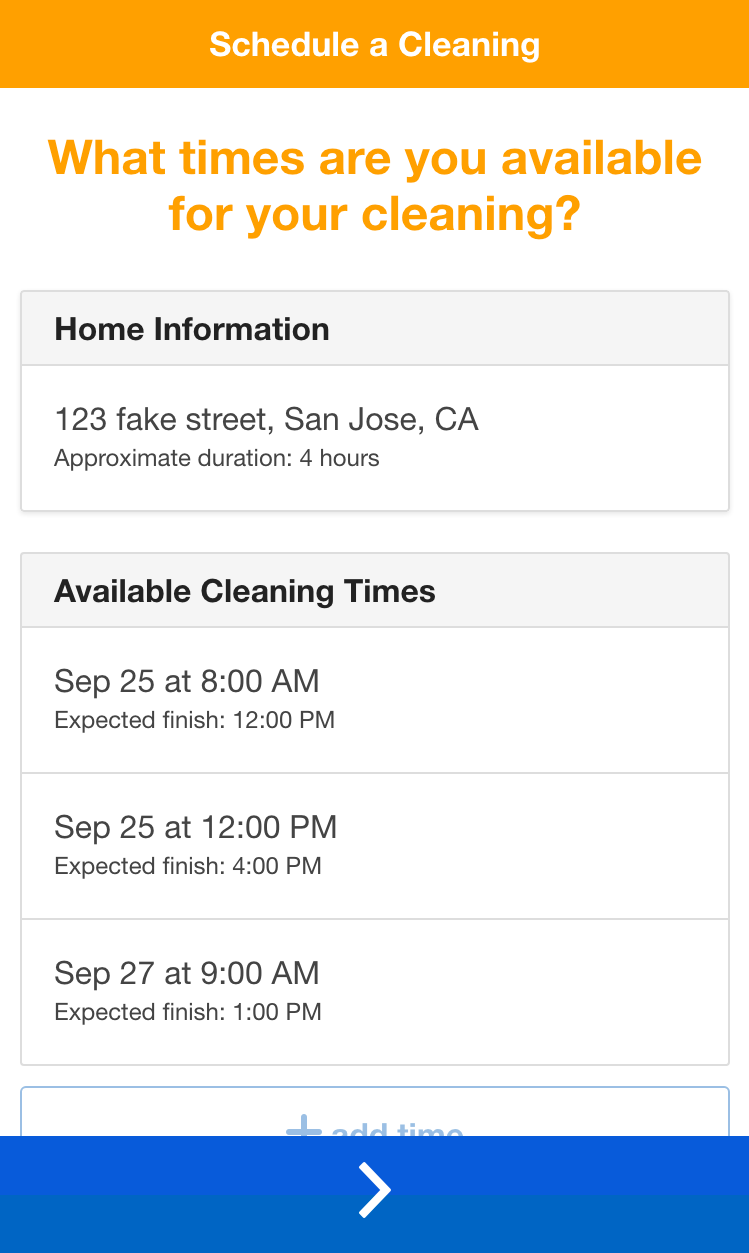
\includegraphics[width=0.25\linewidth]{figures/scheduling}
  %   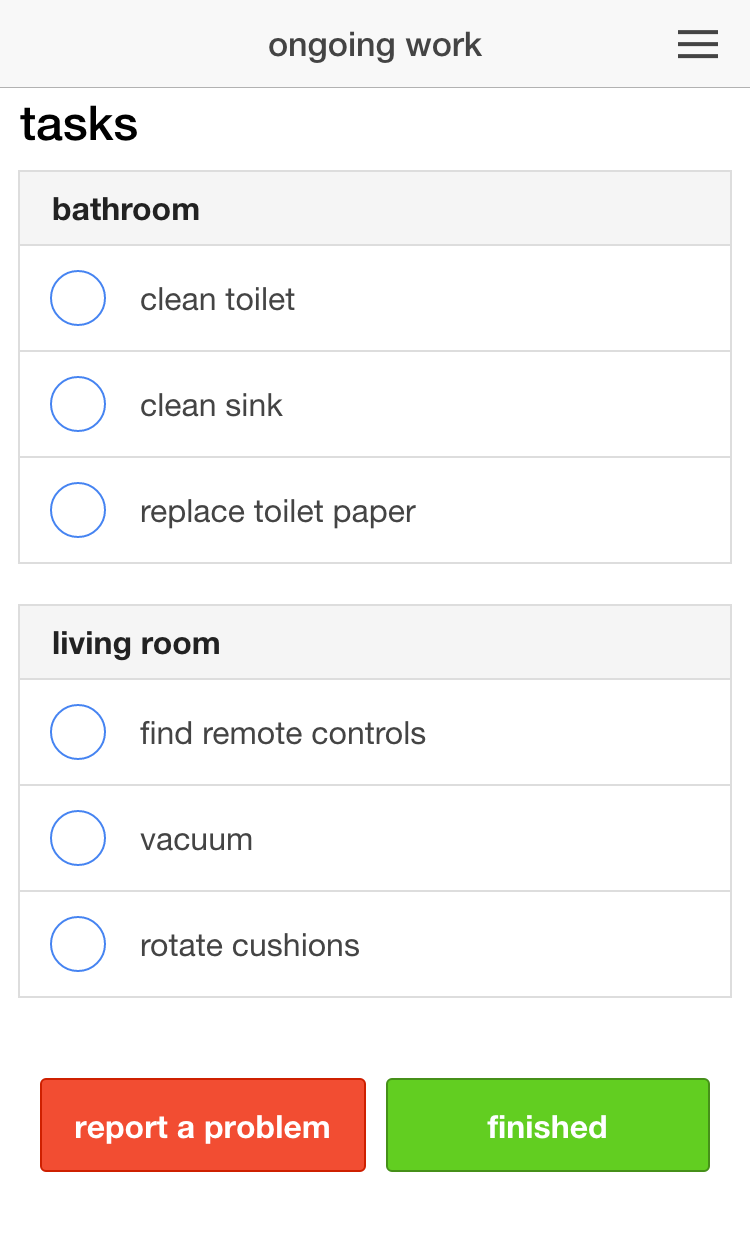
\includegraphics[width=0.25\linewidth]{figures/checklist}
  %   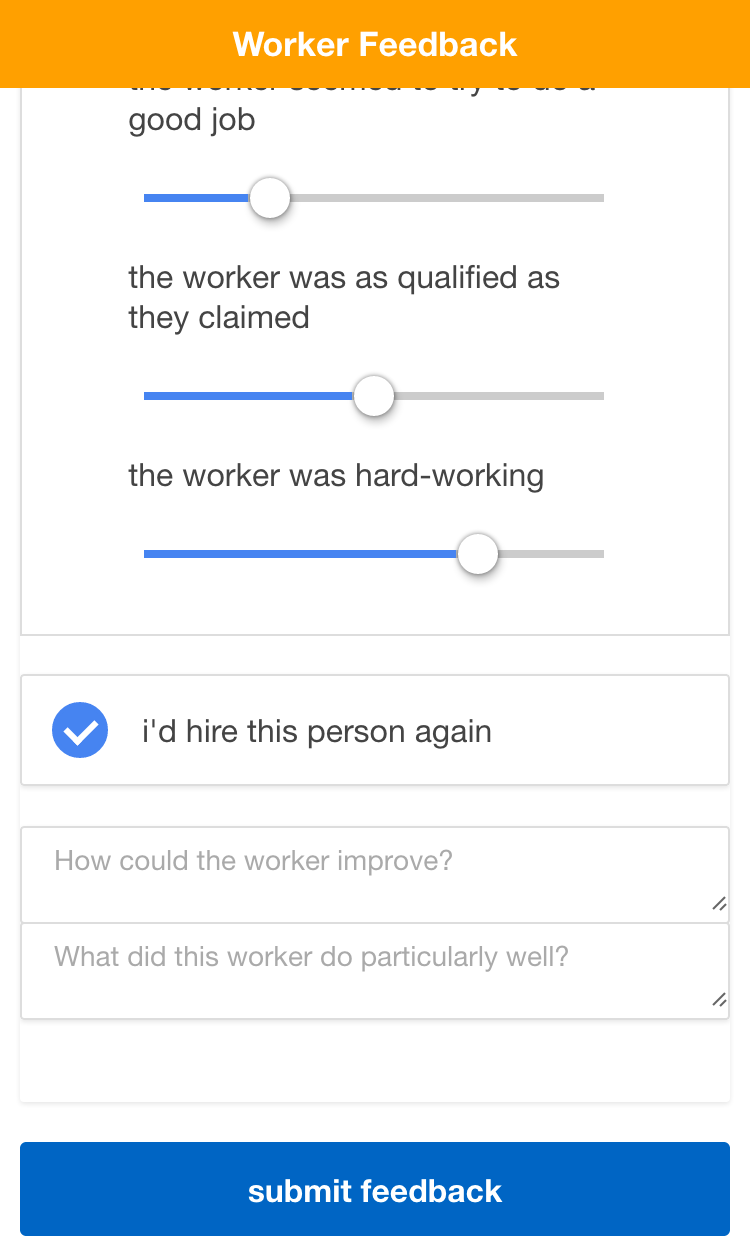
\includegraphics[width=0.25\linewidth]{figures/feedback}
  % \end{figure}
\end{frame}

\section[Moving forward]{Where we're going}
\begin{frame}
  \frametitle{Where we're going}
  \begin{itemize}
    \item Working on \textbf{collective governance}
    \begin{itemize}
      \item Working with a small group of workers
    \end{itemize}
    \item We need to think ahead and build technical system:
    \begin{itemize}
      \item code:
      \href{https://github.com/alialkhatib/workerCoop}{github $\rightarrow$ alialkhatib/workerCoop}
    \end{itemize}
    \item Interested in contributing (to either)?\\
    \textbf{Contact me} --- \href{mailto:ali.alkhatib@cs.stanford.edu}{ali.alkhatib@cs.stanford.edu}
  \end{itemize}
\end{frame}

\section[Questions, etc\ldots]{Wrap--up}
\begin{frame}
  \frametitle{Questions?}
  \begin{itemize}
    \item name: \href{https://ali-alkhatib.com}{Ali Alkhatib}
    \item email: \href{mailto:ali.alkhatib@cs.stanford.edu}{ali.alkhatib@cs.stanford.edu}
    \item twitter: \href{https://twitter.com/_alialkhatib}{@\_alialkhatib}
    \item these slides [pdf]:
    {\footnotesize \url{https://al2.in/media/presentations/PlatformCooperativism.pdf}}
    \item slide source [\LaTeX]:
    {\footnotesize \url{https://al2.in/media/presentations/PlatformCooperativism.tex}}
  \end{itemize}
\end{frame}

\end{document} 